In this section we discuss a theorem about subgroups of direct products of
groups, and describe a consequence for subdirect powers of finite nonabelian
simple groups.  The theorem is a slight generalization of a well-known result
due to Remak, Klein, and Fricke (cf.~Rose~\cite{Rose:1978}, Theorem 
8.19 and Exercise 439).
%,~\cite{Rose:1978:excerpt}). 

Let $T_1, T_2, \dots, T_n$ be a collection of groups and suppose $X$ is a
subgroup of their direct product:
\[
X \leq \prod T_k = T_1 \times T_2 \times \cdots \times T_n.  
\]
Let $\pi_i: \prod T_k \rightarrow T_i$ be the usual projection
epimorphism, and let $\hat{\pi}_i : \prod T_k \rightarrow \prod\limits_{k\neq i} T_k$ denote the
projection of  $\prod T_k$ onto the ``complement'' of $T_i$, which we will
denote by $\hat{T}_i = \prod\limits_{k\neq i}T_k$.
\begin{theorem}
\label{thm:1} If $X, T_i$, and $\hat{T}_i$ are as above, 
 then for all $i=1,\dots, n$, 
  \begin{enumerate}[(i)]
  \item $T_i \cap X \subnormal \pi_i(X) \leq T_i \quad \text{ and } \quad 
\hat{T}_i\cap X \subnormal \hat{\pi}_i(X)\leq \hat{T}_i$,
\item  $(T_1\cap X) \times \cdots \times (T_n\cap X) \subnormal X$, and
\item
$\pi_i(X) /(T_i \cap X)\cong 
X/\left((T_i\cap X) \times (\hat{T}_i\cap X)\right) \cong 
\hat{\pi}_i(X) /(\hat{T}_i\cap X).$
  \end{enumerate}
\end{theorem}
\noindent \underline{Proof sketch:} (coming soon) The case $n=2$ is illustrated in the diagram
in Figure~\ref{fig:theorem}.

\begin{figure}[h]
   \begin{center}
  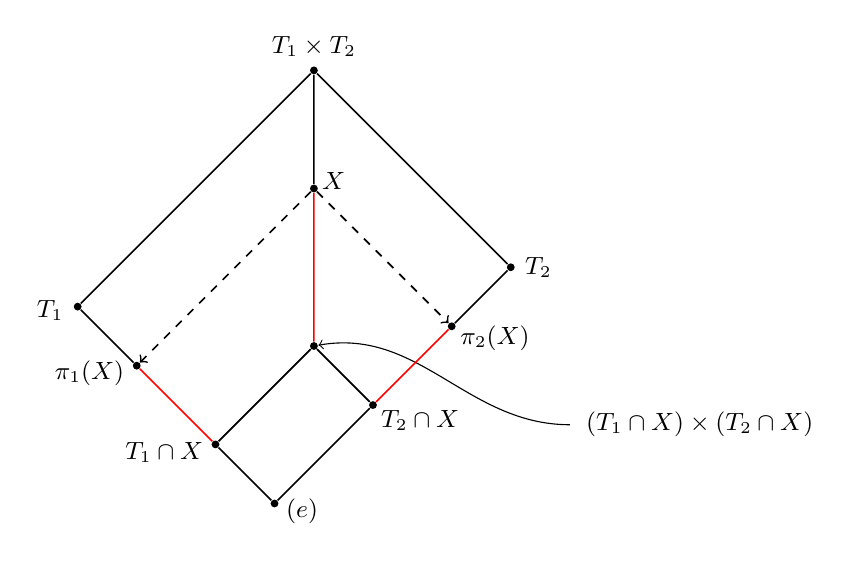
\begin{tikzpicture}[scale=.5]
    \node (e) at (0,0) [fill,circle,inner sep=1pt] {};
    \draw[font=\small] (.7,-.2) node {$(e)$};
    \node (T1capX) at (-1.5,1.5) [fill,circle,inner sep=1pt] {};
    \draw[font=\small] (-2.8,1.3) node {$T_1\cap X$};
    \node (T2capX) at (2.5,2.5) [fill,circle,inner sep=1pt] {};
    \draw[font=\small] (3.7,2.1) node {$T_2\cap X$};
    \node (pi1) at (-3.5,3.5) [fill,circle,inner sep=1pt] {};
    \draw[font=\small] (-4.7,3.3) node {$\pi_1(X)$};
    \node (pi2) at (4.5,4.5) [fill,circle,inner sep=1pt] {};
    \draw[font=\small] (5.6,4.2) node {$\pi_2(X)$};
    \node (Y) at (1,4) [fill,circle,inner sep=1pt] {};
    \draw[->] (7.5,2) to [out=180,in=10] (Y);
    \draw[font=\small] (10.8,2) node {$(T_1\cap X)\times (T_2 \cap X)$};

    \node (X) at (1,8) [fill,circle,inner sep=1pt] {};
    \draw[font=\small] (1.5,8.2) node {$X$};
    \node (T1) at (-5,5) [fill,circle,inner sep=1pt] {};
    \draw[font=\small] (-5.7,4.9) node {$T_1$};
    \node (T2) at (6,6) [fill,circle,inner sep=1pt] {};
    \draw[font=\small] (6.7,6) node {$T_2$};
    \node (T1T2) at (1,11) [fill,circle,inner sep=1pt] {};
    \draw[font=\small] (1,11.6) node {$T_1\times T_2$};


    \draw[semithick]
    (T1T2) to (X)
    (e) to (T1capX) to (Y) to (T2capX) to (e)
    (pi1) to (T1) to (T1T2) to (T2) to (pi2);

    \draw[->, dashed, semithick]
    (X) to (pi1);

    \draw[->, dashed, semithick]
    (X) to (pi2);
    
    \draw[red, semithick]
    (T1capX) to (pi1)
    (T2capX) to (pi2)
    (Y) to (X);
  \end{tikzpicture}
  \caption{Illustrates Theorem~\ref{thm:1} in case $n=2$.  Solid lines
    represent subgroup relations. Intervals colored red are isomorphic. Dashed
    lines emphasize the fact that the projections, $\pi_1(X)$ and
    $\pi_2(X)$, are not generally subgroups of $X$.}  
  \label{fig:theorem}
\end{center}
\end{figure}

Recall, $X$ is a subdirect product of $T_1, \dots, T_n$ provided
 $X \leq \prod\limits_k T_k $ and the projections are onto: $\pi_i(X)= T_i$.  We
denote this situation by  
%$X \stackrel{_{ \mathrm{sd}}}{\hookrightarrow} \prod_i T_i$.
$X \stackrel{_{\mathrm{sd}}}{\leq} \prod T_k$.
%$X \leq_{\mathrm{sd}}\prod_i T_i$.
The following is a consequence of Theorem~\ref{thm:1}:
% and the CFSG theorem:\footnote{The classification of
%finite simple groups (which is a theorem) is called ``the CFSG theorem.''}
\begin{corollary}
  If $T$ is a finite nonabelian simple group and 
$X \stackrel{_{\mathrm{sd}}}{\leq} T^n$,
%$X \stackrel{_{ \mathrm{sd}}}{\hookrightarrow} T^n$,
  then $T \cong X/ (T^{n-1}\cap X)$.  Thus, there are (at least) $n$ distinct normal
  subgroups of $X$ (namely,  $\hat{T}\cap X$) with the property that the
  quotient group is isomorphic to $T$.  In case $n=2$, every subdirect product
  of $T^2$ is isomorphic to $T$.
\end{corollary}
